\section{DNN accelerator: The Need}

The dominant computation of choice in many DNN workloads are either vector-matrix multiplication, matrix-matrix multiplication or convolution. All three operations have high data-parallelism in general and systolic arrays is a better fit for such accelerators. Figure \ref{fig:conv} gives an example and Figure \ref{fig:convcode} is the 7 dimensional loop that represents a convolution.

\begin{figure}[h]
    \centering
    \begin{subfigure}{0.5\textwidth}
        \centering
        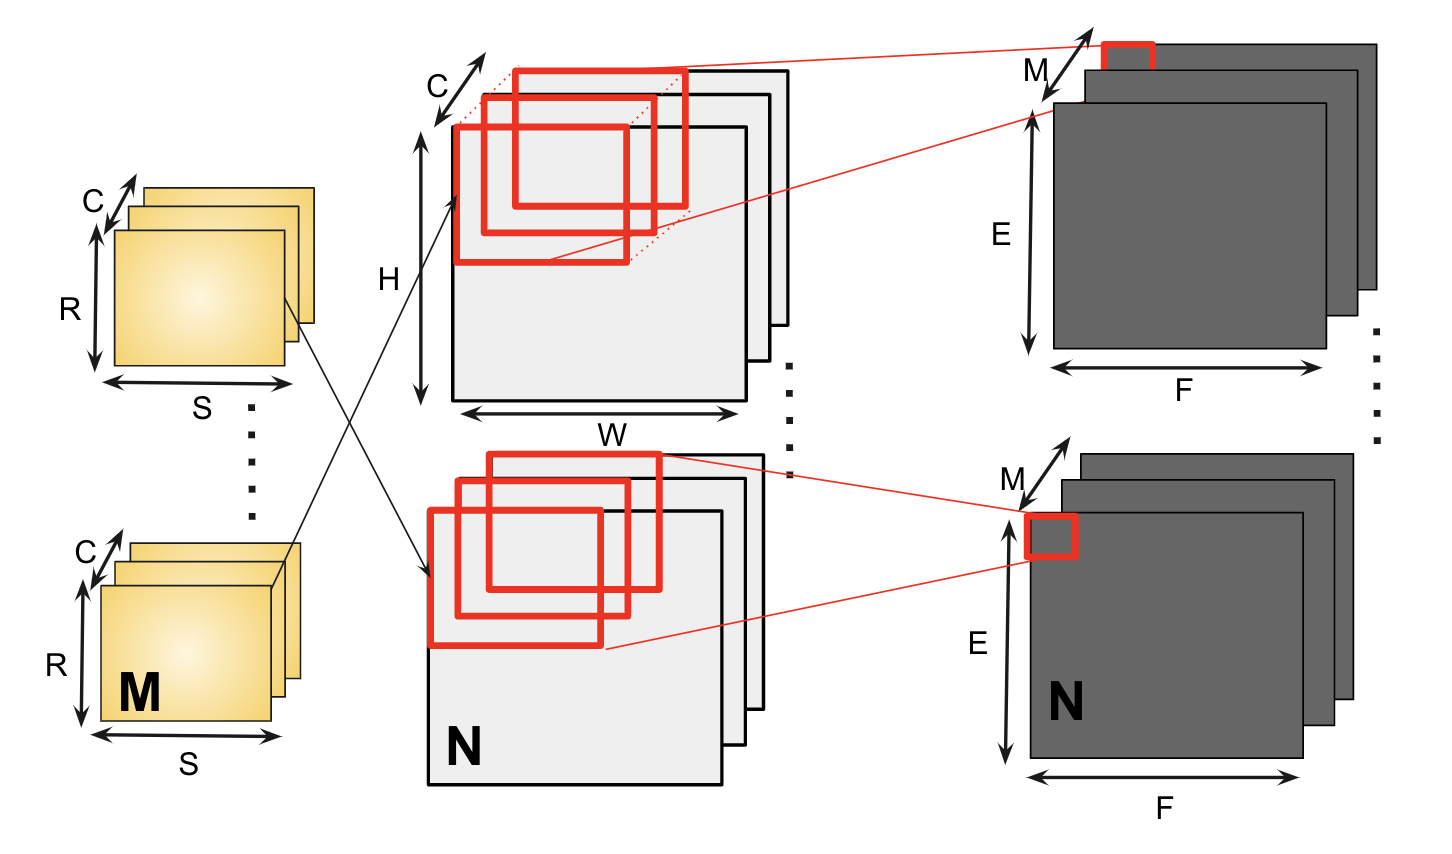
\includegraphics[width=\linewidth]{images/convEx.png}
        \caption{Convolution Operation}
        \label{fig:conv}
    \end{subfigure}%
    \begin{subfigure}{0.5\textwidth}
        \centering 
        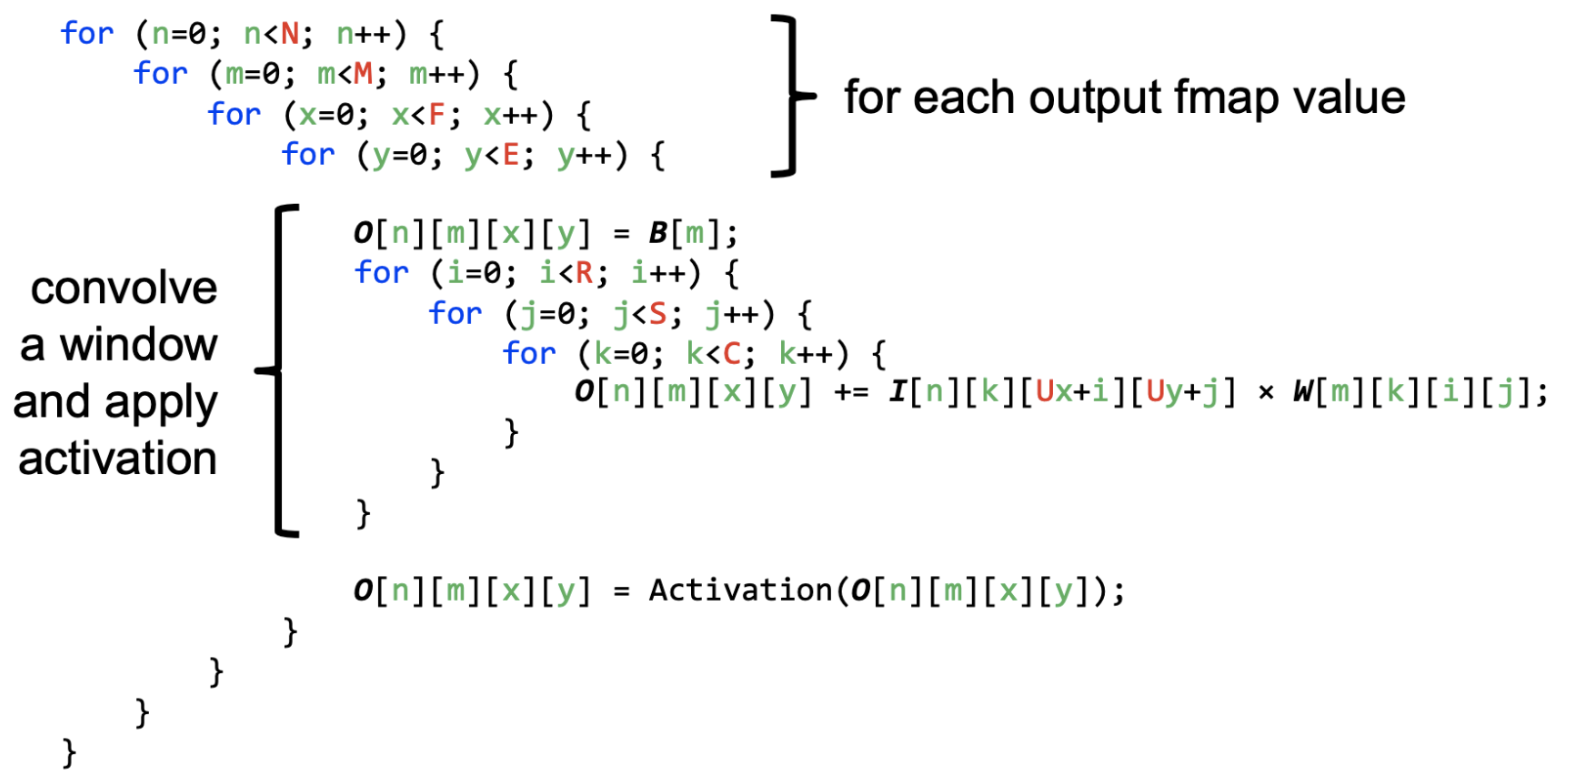
\includegraphics[width=\linewidth]{images/convCode.png}
        \caption{7D convolution code (Courtesy: CS6886 Slides)}
        \label{fig:convcode}
    \end{subfigure}

\end{figure}

% \begin{figure}[h]
%     \centering
%     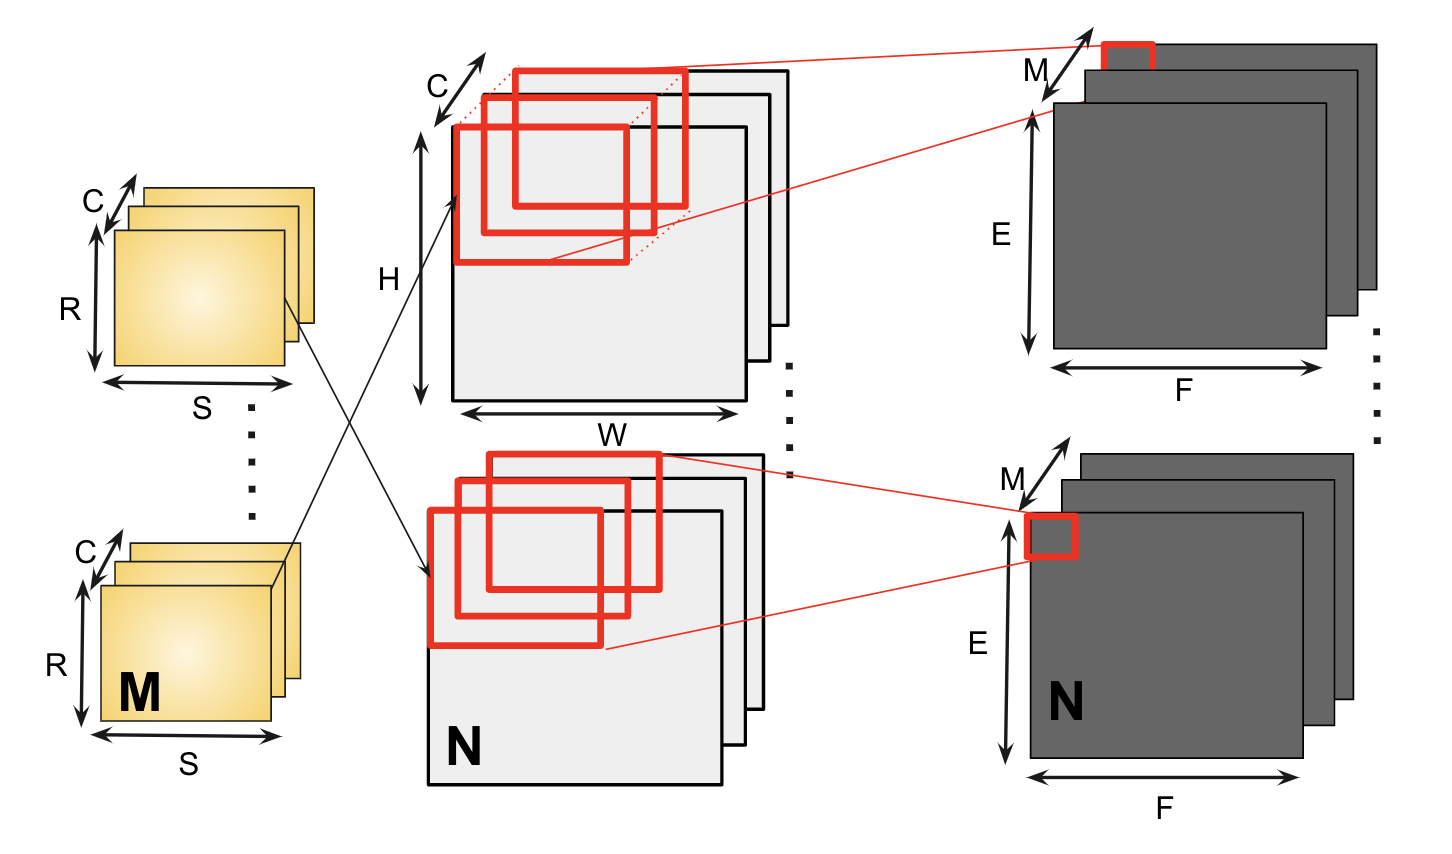
\includegraphics[scale=0.5]{images/convEx.png}
%     \caption{Convolution Operation}
%     \label{fig:conv}
% \end{figure}


% \begin{figure}[h]
%     \centering 
%     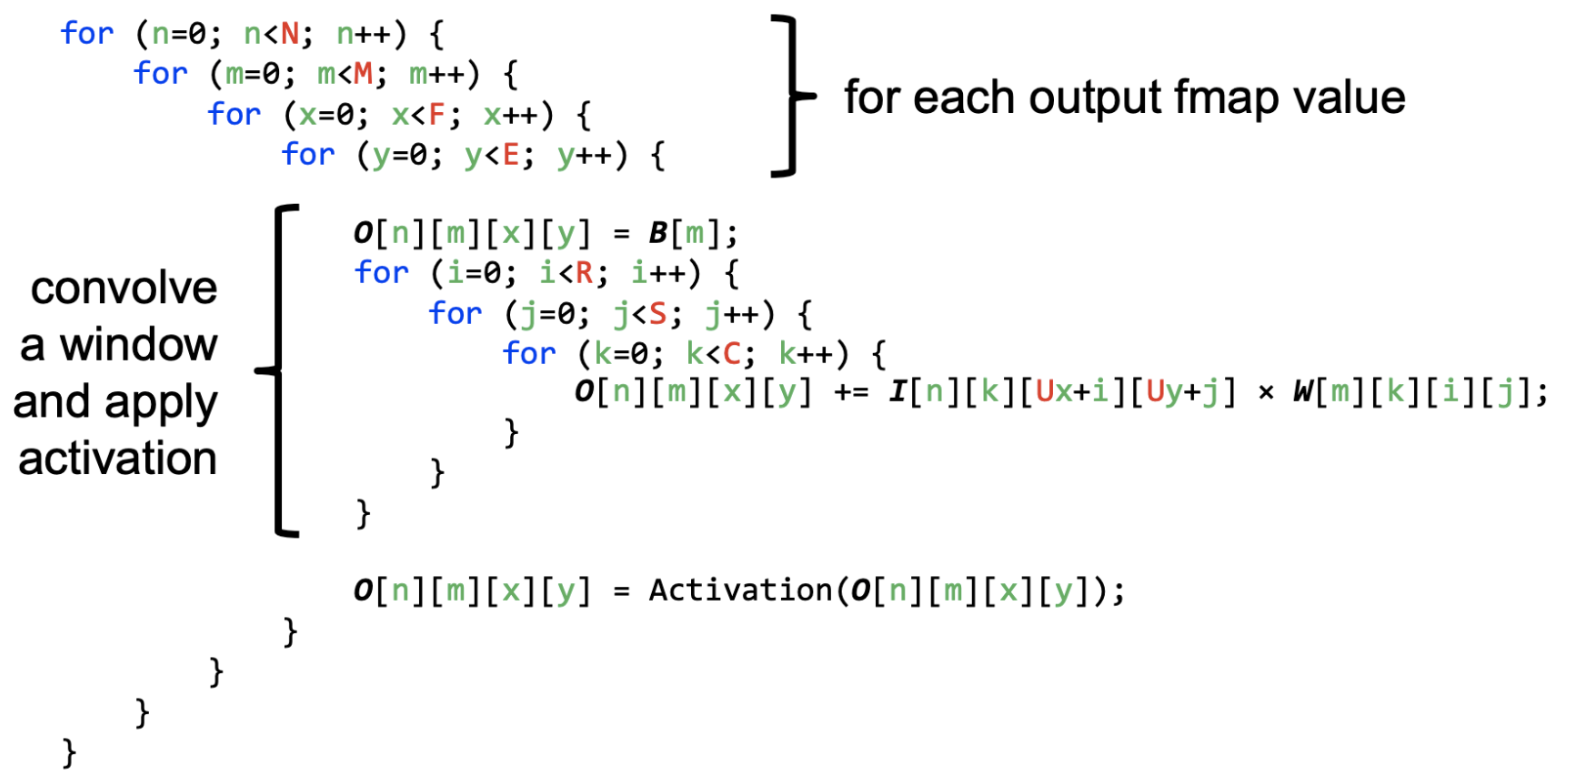
\includegraphics[scale=0.5]{images/convCode.png}
%     \caption{7D convolution code (Courtesy: CS6886 Slides)}
%     \label{fig:convcode}
% \end{figure}

%\section{What's and Why's of Systolic Arrays}
%This question is best answered by the seminal paper from HT Kung and the modern Tensor Processing Unit (TPU).

